\subsection{Reformulation of the search space}

In a talk by Nikolaus Hansen, it was suggested that a source of poor performance 
for the CMA-ES is that the formulation of the problem is ill posed.
He mentioned that if the CMA-ES fails to perform well at optimizing some problems, however a reformulation of the problem could in many cases benefit the CMA-ES. As with the 
MDPTetris platform, the search points are sampled in $\mathbb{R}^n$ where 
$n$ is the number of dimensions. As we saw in section \ref{normalSamples}, the length 
of the sampled vector does not matter, but only the direction. Our experiments also shows that 
the CMA-ES appears to move it's search far away from the origin of the coordinate axis,
which may not be necessary. To overcome this, one might instead choose to search in angles 
of search vectors, and have all search points keep a length of 1. As an example, 
consider a feature set of 3 features. Then a candidate solution has the form of
\begin{align}
x &= \begin{pmatrix}
x_1 \\
x_2 \\
x_3
\end{pmatrix}
\end{align}
Instead of searching arbitraily in $\mathbb{R}^3$, we could search for two angles that rotates
a basis vector in first one coordinate axis, and then another. This way, a search point $p$ 
could be
\begin{align}
p &= \begin{pmatrix}
\theta_0\\
\theta_1
\end{pmatrix}
\end{align}
and the candidate solution $x$
\begin{align}
x &= 
\begin{bmatrix}
cos\left( \theta_0 \right) & sin\left( \theta_0 \right) & 0\\
-sin\left( \theta_0 \right) & cos\left( \theta_0 \right) & 0\\
0 & 0 & 1\\
\end{bmatrix}
\begin{bmatrix}
cos\left( \theta_1 \right) & 0 & -sin\left( \theta_1 \right)\\
0 & 1 & 0\\
sin\left( \theta_1 \right) & 0 & cos\left( \theta_1 \right)
\end{bmatrix}
\begin{pmatrix}
1\\
0\\
0
\end{pmatrix}
\end{align}
Hence, the search space would be reduced by one dimension, and all unique solutions would exist
within $[0; 2 \pi]$ in all dimensions and all candidate solutions would be points on the $n$-dimensional
hypersphere. The idea of this would be to prevent the CMA-ES to search too far off the origin of the
coordinate axis, and instead focus on thoroughly exploring the more confined search space.
The example is illustrated in figure \ref{fig:searchInAngles}

\begin{figure}[H]
\begin{center}
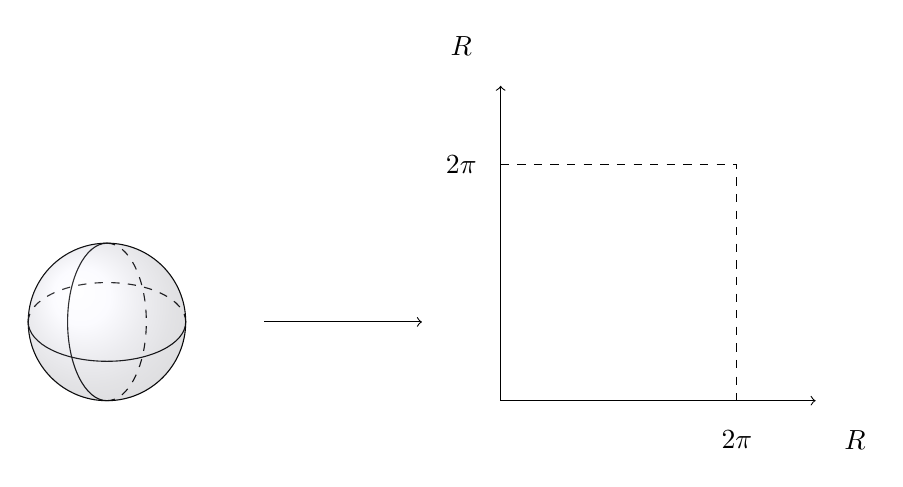
\begin{tikzpicture}
    \draw (-1,0) arc (180:360:1cm and 0.5cm);
    \draw[dashed] (-1,0) arc (180:0:1cm and 0.5cm);
    \draw (0,1) arc (90:270:0.5cm and 1cm);
    \draw[dashed] (0,1) arc (90:-90:0.5cm and 1cm);
    \draw (0,0) circle (1cm);
    \shade[ball color=blue!10!white,opacity=0.20] (0,0) circle (1cm);
    \draw[->] (2,0) -- (4,0);
\draw[->] (5,-1) node (v1) {} -- (5,3);
\draw[->] (5,-1) -- (9,-1);
\draw[dashed] (5,2) -- (8,2) -- (8,-1);
\node at (4.5,3.5) {$\mathbb{R}$};
\node at (9.5,-1.5) {$\mathbb{R}$};
\node at (4.5,2) {$2\pi$};
\node at (8,-1.5) {$2\pi$};
\end{tikzpicture}
\end{center}
\caption{Illustration of the 3-dimensional hypersphere, with a search space of $\mathbb{R}^2$
\label{fig:searchInAngles}}
\end{figure}


